\section{Lyons p. 3.12}

Lad $ \left(x(n) \in \sets{x(n) : 0 < n \le N, N \in \N} \right) $ være en tidsserie af størrelse $ N $,
for hvilket det gælder at $ \left( \mathcal{X}(m) : 0 \le m \le N - 1 \right) $ representere den diskrete fourier transformation 
afs$ x(n) $ som beskrevet af ligning~\eqref{eq:DFT-def}.

\begin{align}
  \label{eq:DFT-def}
  \mathcal{X}(m) = \sum_{n = 0}^{N - 1} x(n)\exp\sets{-\frac{j2 \pi nm}{N}}.
\end{align}

Tag i betragtning påstanden fra ligning~\eqref{eq:claim3.12} og hvis hvorvidt denne påstand er sand eller falsk. 

\begin{align}
  \label{eq:claim3.12}
  \sum_{m = 0}^{N-1} \mathcal{X}(m) = Nx(n), \quad n = 0.
\end{align}

\begin{proof}
  Tag i betragtning den inverse fourier transformation, givet ved ligning~\eqref{eq:inverseDFT}.

  \begin{align}
    \label{eq:inverseDFT}
    x(n) &= \frac{1}{N} \sum_{m = 0}^{N - 1} \mathcal{X}(m) \exp\sets{\frac{j 2 \pi n m}{N}}, \\
         &\Updownarrow (n = 0) \\
    x(0) &= \frac{1}{N} \sum_{m = 0}^{N - 1} \mathcal{X}(m), \\
         &\Updownarrow \\
    Nx(0) &= \sum_{m = 0}^{N - 1} \mathcal{X}(m)
  \end{align}
\end{proof}

Det er dermed vist at påstanden, fremført i ligning~\eqref{eq:claim3.12}, er sand.

\newpage

\section{Lyons p. 3.15}

Tag i betragtning et datasæt, $ N = 902 $, for en tidsserie $ x(n) $. Datasættet er samplet med
frekvens $ f_{s} = 22.225\ kHz $. \autoref{fig:spectData} viser den discrete fourier transformation
af $ x(n) $ over frekvens indekset $ 0 \le m \le 59 $.

\begin{figure}[h]
  \centering
  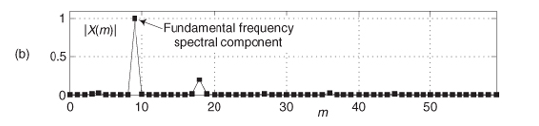
\includegraphics[width = \textwidth]{figures/SampleMag.png}
  \caption{Spectral Magnitude Sample}%
  \label{fig:spectData}
\end{figure}

Baset på $ \mathcal{X}(m) $ samples hvad er grundfrekvensen, i Hertz? 
Dette er givet ved brug af ligningen~\eqref{eq:fAnalysis}

\begin{align}
  \label{eq:fAnalysis}
  f_{analysis} = \frac{mf_{s}}{N}.
\end{align}

Det kan aflæses på \autoref{fig:spectData} grundfrekvensen til hører bin $ m = 9 $.
Grundfrekvensen er da givet som
  
\begin{align}
  f_{9} &= \frac{9 f_{s}}{N} \\
        &= \frac{9 \cdot 22.255 kHz}{902} \\
        &= 222.057 Hz
\end{align}

Givet, istedet, en logaritmisk scaling, se \autoref{fig:logSpectData}, hvad er frekvensen for det højste Spectral komponent, forskelligt fra $0$?

\begin{figure}[h]
  \centering
  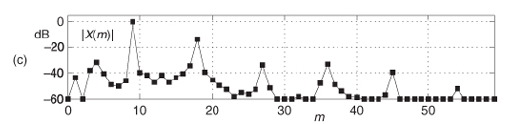
\includegraphics[width = \textwidth]{figures/LogSampleMag.png}
  \caption{Spectral Magnitude Sample}%
  \label{fig:logSpectData}
\end{figure}

Her benyttes igen ligning~\eqref{eq:fAnalysis} hvor med $ m = 18 $ aflest fra~\autoref{fig:logSpectData}, hvorved der fås at

\begin{align}
  f_{18} &= \frac{18f_s}{N} \\
         &= \frac{18 \cdot 22.255 kHz}{902} \\
         &= 444.113 Hz
\end{align}

\newpage

\section{Lyons p. 4.1}
Givet et datasæt, af størrelse $N$ samples, Hvilket forskelle er der på resultat af DFT og FFT?%

Der er ingen forskell på DFT og FFT iforhold til hvor præcise de er i deres udregninger.
Den store forskell på de to ``algoritmer'' er at tidskompleksiteten for DFT og FFT er 
$\mathcal{O}(n^{2})$ hvorimod for FFT er den $\mathcal{O}(n\log{n})$. Dette betyder at FFT
på store datasæt kan udføres utroligt hurtigt. På små datasæt er der ikke den store forskell
tidsmæssigt på udførelsen af de to algoritmer.

FFT har en restriktion dog. Den antager at sample size er et multiplum af 2. Altså at $N = k^{2}, k \in \N$.


